\newpage
\subsubsection{UC3 - Configurazione del plug-in}
\label{sssec:uc3}

\begin{figure}[h!]
  \begin{center}
    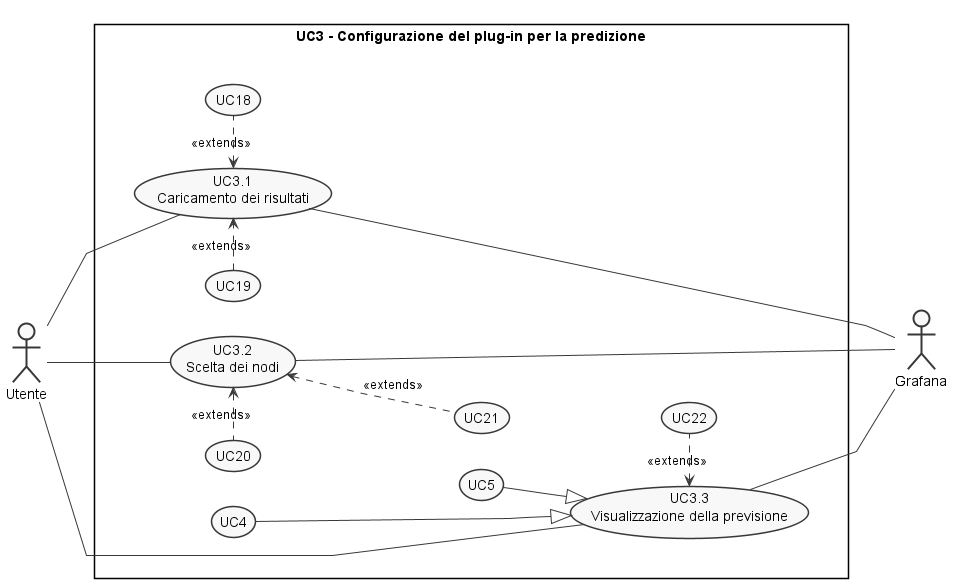
\includegraphics[width=12cm]{uc3.png}\\
    \caption{UC3 - Configurazione del plug-in}%
    \label{fig:uc3}
  \end{center}
  \end{figure}

\begin{description}
  \item[Attore primario]: Utente amministratore.
  \item[Attore secondario]: Grafana.
  \item[Descrizione:] Configurazione del plug-in per ottenere delle previsioni.
  \item[Precondizione:] L'amministratore ha abilitato il plug-in e si trova nella pagina di configurazione.
  \item[Scenario principale:]
  \begin{enumerate}
    \item L'amministratore carica il file JSON contente i risultati dell'addestramento (UC3.1);
    \item L'amministratore sceglie su quali nodi fare le previsioni (UC3.2);
    \item L'amministratore sceglie con quale modalità visualizzare i dati (UC3.3).
  \end{enumerate}
  \item[Postcondizione:] L'amministratore ha configurato il plug-in, il quale diventa pronto per essere avviato.
\end{description}

\paragraph{UC3.1 - Caricamento risultati}
\label{sssec:uc3.1}
\begin{description}
  \item[Attore primario:] Utente amministratore.
  \item[Descrizione:] L'amministratore carica il file JSON contenente i risultati ottenuti dall'addestramento.
  \item[Precondizione:] L'amministratore ha a disposizione un file con all'interno i risultati (UC1.5).
  \item[Scenario principale:] L'amministratore carica il file JSON contenente i risultati ottenuti dall'addestramento.
  \item[Postcondizione:] L'amministratore ha caricato il file contenente i risultati dell'addestramento avvenuto precedentemente.
  \item[Estensioni:]
  \begin{enumerate}
	\item UC3.1 viene esteso nel caso d'uso UC9 con la visualizzazione del messaggio di errore quando viene fornito un predittore in un formato non valido;
	\item UC3.1 viene esteso nel caso d'uso UC10 con la visualizzazione del messaggio di errore quando l'amministratore non inserisce alcun file per l'addestramento.
  \end{enumerate}
\end{description}

\paragraph{UC3.2 - Scelta dei nodi}
\label{sssec:uc3.2}
\begin{description}
  \item[Attore primario:] Utente amministratore.
  \item[Descrizione:] L'amministratore sceglie su che nodi effettuare la previsione.
  \item[Precondizione:] L'amministratore ha il file di dati di addestramento (UC3.1).
  \item[Scenario principale:] L'amministratore, data una lista di nodi, seleziona quali vuole aggiungere alla predizione.
  \item[Postcondizione:] L'amministratore ha selezionato i nodi da aggiungere alla predizione.
  \item[Estensioni:]
  \begin{enumerate}
	\item UC3.1 viene esteso nel caso d'uso UC11 con la visualizzazione del messaggio di errore quando non viene selezionato nessun nodo valido;
	\item UC3.1 viene esteso nel caso d'uso UC12 con la visualizzazione del messaggio di errore quando non viene selezionato alcun nodo.
  \end{enumerate}
\end{description}

\paragraph{UC3.3 - Scelta della modalità di visualizzazione}%
\label{sssec:uc3.3}

\begin{figure}[h!]
  \begin{center}
    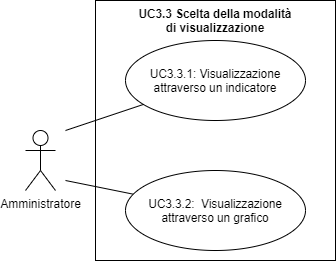
\includegraphics[width=10cm]{uc3.3.png}\\
    \caption{UC3.3 - Scelta della modalità di visualizzazione}%
    \label{fig:uc3.3}
  \end{center}
\end{figure}

\begin{description}
  \item[Attore primario:] Utente amministratore.
  \item[Descrizione:] L'amministratore seleziona il tipo di visualizzazione.
  \item[Precondizione:]  L'amministratore ha selezionato i nodi da utilizzare per la previsione (UC3.2).
  \item[Scenario principale:] L'amministratore sceglie se visualizzare i dati generati dalla previsione per mezzo di un indicatore o di un grafico.
  \item[Postcondizione:] L'amministratore ha scelto che modalità di visualizzazione usare.
  \item[Estensioni:] UC3.3 viene esteso nel caso d'uso UC13 con la visualizzazione del messaggio di errore quando non viene scelta una modalità di visualizzazione.
\end{description}

\subparagraph{UC3.3.1 - Visualizzazione attraverso un indicatore}
\label{sssec:uc3.3.1}
\begin{description}
  \item[Attore primario:] Utente amministratore.
  \item[Descrizione:] L'indicatore viene scelto come modalità di visualizzazione dei dati.
  \item[Precondizione:] L'amministratore ha a disposizione le due modalità.
  \item[Scenario principale:] L'amministratore sceglie l'indicatore per visualizzare i dati generati dalla previsione.
  \item[Postcondizione:] L'amministratore ha deciso di utilizzare l'indicatore.
\end{description}

\subparagraph{UC3.3.2 - Visualizzazione attraverso un grafico}
\label{sssec:uc3.3.2}
\begin{description}
  \item[Attore primario:] Utente amministratore.
  \item[Descrizione:] Il grafico viene scelto come modalità di visualizzazione dei dati.
  \item[Precondizione:] L'amministratore ha a disposizione le due modalità.
  \item[Scenario principale:] L'amministratore sceglie il grafico per visualizzare i dati generati dalla previsione.
  \item[Postcondizione:] L'amministratore ha deciso di utilizzare il grafico.
\end{description}
